\subsubsection{Motivation I: Data Compression}
\begin{itemize}[--]
	\item Lets say we are given a data set, where 2 features are redundant (inches and cm), and we want to reduce the set to only account for 1 copy of this feature
	\item We can think of this reduction, as specifing the distance along the line that these dimensions chart

	\begin{center}
		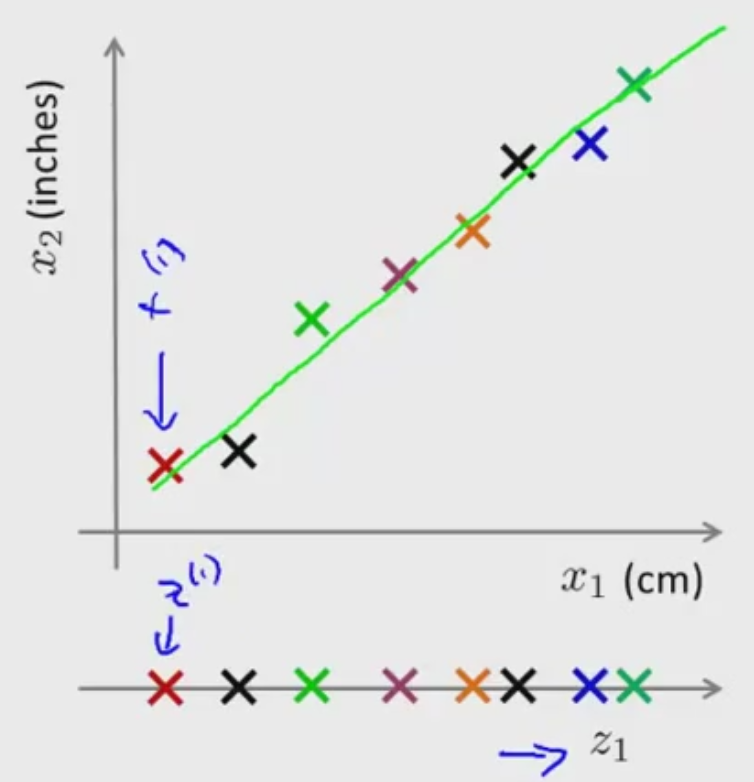
\includegraphics[scale=0.5]{sections/cs229/w11/2d_1d.png}
	\end{center}

	\item Here $z_1$ represents both $x_1$ and $x_2$
	\item This compression can happen from $m$-dimension to $n$-dimension ($m> n$), and is not limited to just one case
\end{itemize}

\subsubsection{Motivation II: Visualization}
\begin{itemize}[--]
	\item For a lot of problems, we want some way to visualize and understand the data 
	\item For example given $x^{(i)}\in\mathbb{R}^{50}$, using dimensionality reduction, we come up with a different feature representation $Z^{(i)}\in\mathbb{R}^2$ where these are some measure of the rest of the dimensions. Now we can chart this in on a plane.
\end{itemize}

\subsubsection{Principal Component Analysis Problem Formulation}
\begin{itemize}[--]
	\item PCA finds a lower dimensional surface on which to project the data, which minizes the projection error (distance from point to surface)
	\begin{center}
		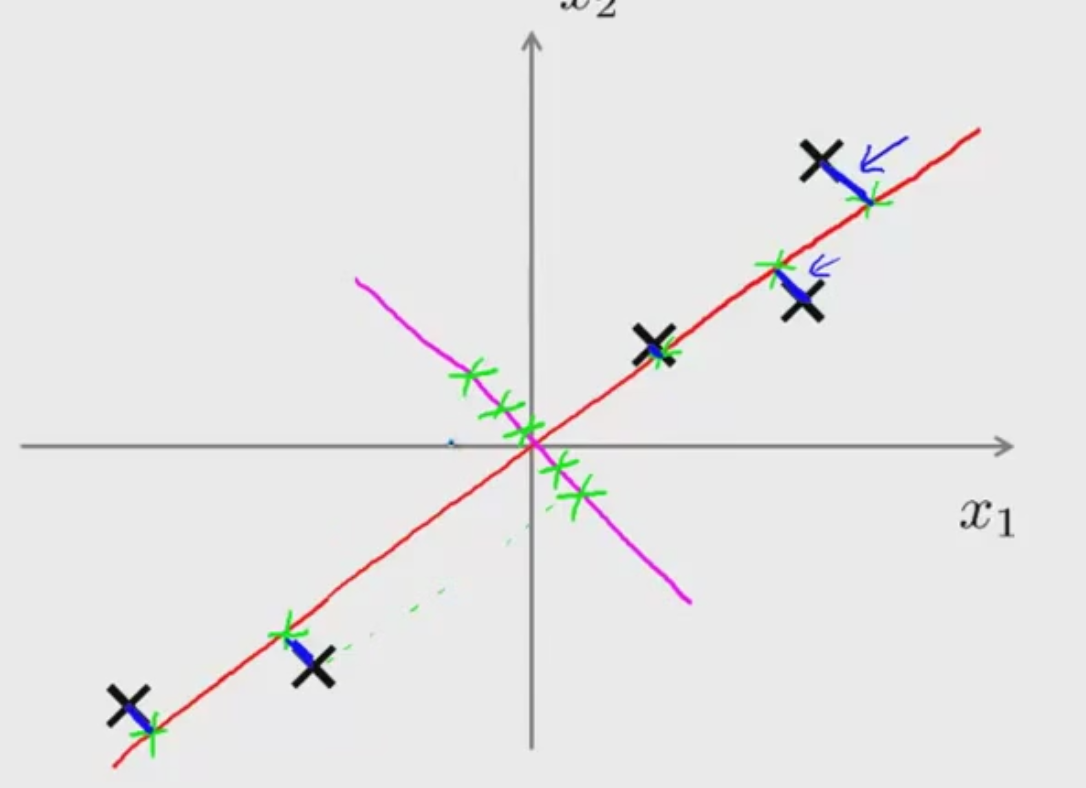
\includegraphics[scale=0.5]{sections/cs229/w11/bad.png}
	\end{center}

	\item There are bad choices (purple line) which have a very large error, and are not a good idea to reduce to, which is why we want to keep the error near zero
	\item \textbf{PCA}: Reduce from $n$-dimension to $k$-dimension: Find $k$ vectors $u^{(1)},\ldots,u^{(k)}$ onto which to project the data, so as to minimze the projection error
\end{itemize}

\subsubsection{Principal Component Analysis Algorithm}
\begin{itemize}[--]
	\item Data preprocessing
	\begin{itemize}[--]
		\item Training set: $x^{(1)},\ldots, x^{(m)}$
		\item Preprocessing (feature scaling/mean normalization);
			$$\mu_j = \frac{1}{m}\sum_{i=1}^{m}x_j^{(i)}$$
		\item Replace $x_j^{(i)}$ with $x_j - \mu_j$
		\item If different features on different scales (eg., $x_1=$size of house, $x_2=$ number of bedrooms), scale features to have comparable range of values
	\end{itemize}

	\item Reduce data from $n$-dimensions to $k$-dimensions
	\item Compute ``Covariance matrix'':
		$$\sigma = \frac{1}{m}\sum_{i=1}^{n} (x^{(i)})(x^{(i)})^T$$
	\item Compute eigenvectos of matrix $\sigma$: $[U, S, V] = svd(Sigma);$
	\item The $U$ matrix will have columns of the principal components $[u^{(i)}]$, since $U\in\mathbb{R}^{n\times n}$ we only need to take the first $k$ columns to reduce
		$$x\in\mathbb{R}^n\to z\in\mathbb{R}^k$$
		$$z= [\vec{u^{(1)}}, \ldots, \vec{u^{(k)}}]^{T} x $$
\end{itemize}

\subsubsection{Choosing the Number of Principal Components}
\begin{itemize}[--]
	\item Average squared projection error: $\frac{1}{m}\sum_{i=1}^{m} ||x^{(i)}- x_{approx}^{(i)} ||^2$
	\item Total variation in the data: $\frac{1}{m}\sum_{i=1}^{m}||x^{(i)}||^2$
	\item Typicall, choose $k$ to be the smallest value so that:
		$\frac{\text{Average squared proj error}}{\text{Total variation in data}}\leq 0.01$
	\item ``99\% of variance is retained''
	\item Algorithm:
	\begin{itemize}[--]
		\item Try PCA with $k=1:n$
		\item Compute $U_{reduce}, z^{(1)}, \ldots, z^{(m)}, x^{(1)}_{approx},\ldots, x^{(m)}_{approx}$
		\item Check if: $\leq 0.01$
	\end{itemize}

	\item When computing $[U, S, V]$, where $S$ is the diagonal matrix of eigenvalues
	\item For a given k:
		$$1-\frac{\sum_{i=1}^{k} S_{ii}}{\sum_{i=1}{n} S_{ii}}\leq 0.01$$
	\item This will give us the variability fraction like above
\end{itemize}

\subsubsection{Reconstrction from Compressed Representation}
\begin{center}
	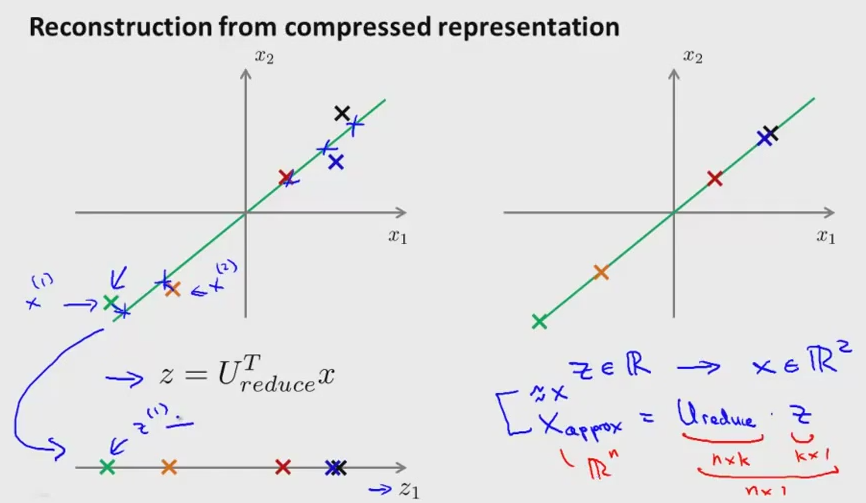
\includegraphics[scale=0.5]{sections/cs229/w11/reduce.png}
\end{center}
 
\subsubsection{Advice for Applying PCA}
\begin{itemize}[--]
	\item Suppose we have $(x^{(m)}, y^{(m)})$, $x^{(i)}\in\mathbb{R}^{10000}$ like in computer vision algorithms, running a learning algorithm will be very slow
	\item First extract inputs:
	\begin{itemize}[--]
		\item Unlabeled dataset: $x^{(1)},\ldots, x^{(m)}\in\mathbb{R}^{10000}$
		\item We convert via PCA into: $z^{(1)},\ldots, z^{(m)}\in\mathbb{R}^{1000}$
	\end{itemize}
	\item Now we have: $(z^{(1)}, y^{(1)})$, because our training examples are now represented with a lower dimension input
	\item Then we will learn our hypothesis: $h(z)$
	\item You should only reduce the training set, not the cv or test sets
	\item Bad use of PCA: To prevent overfitting:
	\begin{itemize}[--]
		\item Use $z^{(i)}$ instead of $x^{(i)}$ to reduce the number of features to $k < n$
		\item Thus, fewer features, less likely to overfit
		\item This might work OK, but isn't a good way to address overfitting. User regularization instead.
	\end{itemize}

	\item Consider, doing the whole thing without using PCA
	\item Before implementing PCA, first try running whatever you want to do with the original/raw data $x^{(i)}$. Only if that doesn't do what you want, then implement PCA and consider using $z^{(i)}$.

\end{itemize}
